% Physics experiment report
% 9/Dec/2016

\documentclass[a4paper,12pt,notitlepage]{article}

\usepackage{CJKutf8}
\usepackage{amsmath}
\usepackage{indentfirst}
\usepackage{graphicx}
\usepackage{longtable}

\setlength{\parindent}{2em} 

\begin{CJK*}{UTF8}{gbsn}
\begin{document}

\title{刚体转动实验报告}
\author{秦光辉\ 9组3号}
\maketitle

\section{实验数据处理}

\subsection{实验内容一}

	每个实验重复三次, 每次实验时线轴半径均为2.50cm, 两个柱体都位于$x_5$处, 实验数据如表一所示.
	
\begin{center}
	\begin{longtable}{|c|c|c|c|c|c|c|c|c|c|c|c|c|}

	\caption{第一组实验数据}	\\
	\hline
	m/g & $t_1$/s & $t_2$/s & $t_3$/s & $\bar{t}$/s & $\frac{1}{\bar{t}^2}$/$s^{-2}$ \\
	\hline
	5.00 & 17.22 & 17.16 & 17.18 & 17.19 & 0.00339 \\
	\hline
	10.00 & 11.44 & 11.53 & 11.50 & 11.49 & 0.00758 \\
	\hline
	15.00 & 9.09 & 9.27 & 9.09 & 9.15 & 0.01194 \\
	\hline
	20.00 & 7.78 & 7.90 & 7.84 & 7.84 & 0.01627 \\
	\hline
	25.00 & 6.85 & 6.97 & 7.00 & 6.94 & 0.02076 \\
	\hline
	30.00 & 6.37 & 6.25 & 6.40 & 6.34 & 0.02488 \\
	\hline
	35.00 & 5.97 & 5.91 & 5.94 & 5.94 & 0.02834 \\
	\hline

	\end{longtable}
\end{center}

	实验中测得砝码下落的高度h为
	
\begin{align*}
	h &= 86.90cm \\
	e_h &= 0.1cm \\
	\sigma_h &= \frac{e_h}{\sqrt{3}} = 0.0577cm
\end{align*}

	考虑到m的误差相对较小, 我们把m当做自变量, 线性拟合直线, 可以得到($r'$为线性回归系数)
	
\begin{align*}
	k &= 8.4454 \times 10^{-4} s^{-2}g^{-1} \\
	b &= -7.35 \times 10^{-4} s^{-2} \\
	r' &= 0.99950 	
\end{align*}

	作图如图一. \\
	
\begin{figure}[h]
\centering
	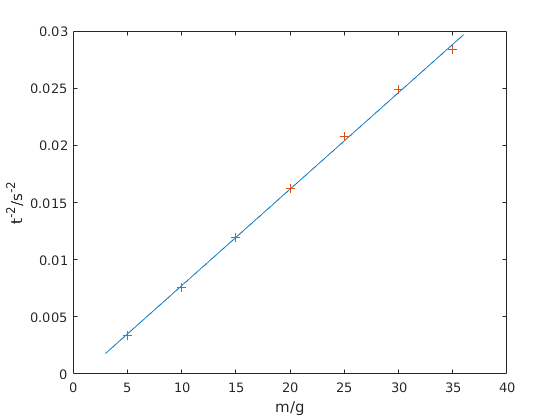
\includegraphics[scale=0.7]{figure_1.png}
	\caption{$t^{-2} - m$关系图}
\end{figure}

	相对于t的误差而言, 实验中m的误差可以忽略不计. 虽然秒表的精度足够高, 但是由于无法准确记录释放和落地时间, 导致时间t的误差非常大, 估计为0.1s. 则
	
\begin{align*}
	\sigma_{t^{-2}} &= -\frac{2\sigma_t}{t^3} \\
	\sigma_k' &= \sqrt{\sum_{i = 1}^n(\frac{\partial k}{\partial t^{-2}})^2} \\
	&= \sqrt{\sum_{i = 1}^n[\frac{m_i - \bar{m}}{\sum_i^n(m_i - \bar{m})^2}\frac{2\sigma_t}{t_i^3}]^2} \\
	&= 9.868 \times 10^{-6} s^{-2}g^{-1} \\
	\sigma_k'' &= k\cdot \sqrt{\frac{1/r'^2 - 1}{n -2}} = 1.195 \times 10^{-5} s^{-2}g^{-1} \\
	\sigma_k &= \sqrt{(\sigma_k')^2 + (\sigma_k'')^2} = 1.5\times 10^{-5} s^{-2}g^{-1}
\end{align*} 

	可以得到转动惯量为
	
\begin{align*}
	I &= \frac{gr^2}{2hk} = 4.173\times 10^{-3} kg \cdot m^2 \\
	\sigma_I &= \sqrt{(\frac{\sigma_k}{k})^2+(\frac{\sigma_h}{h})^2} \cdot I =  0.076 \times 10^{-3} kg\cdot m^2 \\
	I \pm \sigma_I &= (4.17 \pm 0.08) \times 10^{-3} kg\cdot m^2
\end{align*}

\subsection{实验内容二}

	实验二中保持柱体位于$x_5$处, 质量保持
	
\begin{align*}
	m &= 20.00 g \\
\end{align*}

	实验数据见表二. \\
	
\begin{center}
	\begin{longtable}{|c|c|c|c|c|c|c|c|c|c|c|c|c|}

	\caption{第二组实验数据}	\\
	\hline
	r/cm & $t_1$/s & $t_2$/s & $t_3$/s & $\bar{t}$/s & $\frac{1}{\bar{t}^2r}$/$s^{-2}cm^{-1}$ \\
	\hline
	1.00 & 20.16 & 20.25 & 20.34 & 20.25 & 0.002439 \\
	\hline
	1.50 & 13.16 & 13.16 & 13.19 & 13.17 & 0.003844 \\
	\hline
	2.00 & 10.18 & 10.09 & 10.06 & 10.11 & 0.004892 \\
	\hline
	2.50 & 8.09 & 7.97 & 7.91 & 7.99 & 0.006266 \\
	\hline
	3.00 & 6.63 & 6.55 & 6.56 & 6.58 & 0.007699 \\
	\hline

	\end{longtable}
\end{center}
	
	考虑到r的误差相对较小, 我们把r当做自变量, 线性拟合直线, 可以得到($r'$为线性回归系数)
	
\begin{align*}
	k &= 2.5884 \times 10^{-3} s^{-2}cm^{-2} \\
	b &= -1.49 \times 10^{-4} s^{-2}cm^{-1} \\
	r' &= 0.99879
\end{align*}

	拟合直线见图二. \\
	
\begin{figure}[h]
\centering
	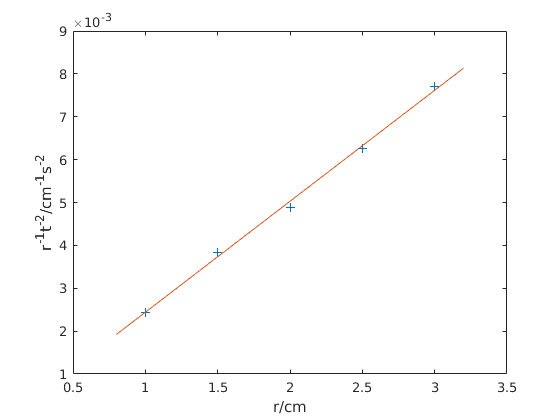
\includegraphics[scale=0.7]{figure_2.png}
	\caption{$t^{-2}r^{-1}-r$关系图}
\end{figure}

	类似于上一个实验的处理, 把时间的不确定度近似取为0.1s, 则有
	
\begin{align*}
	\sigma_{t^{-2}} &= -\frac{2\sigma_t}{t^3} \\
	\sigma_k' &= \sqrt{\sum_{i = 1}^n(\frac{\partial k}{\partial (r^{-1}t^{-2})})^2} \\
	&= \sqrt{\sum_{i = 1}^n[\frac{r_i - \bar{r}}{\sum_i^n(r_i - \bar{r})^2}\frac{2\sigma_t}{r_i t_i^3}]^2} \\
	&= 1.41 \times 10^{-4} s^{-2}cm^{-2} \\
	\sigma_k'' &= k\cdot \sqrt{\frac{1/r'^2 - 1}{n -2}} = 7.358 \times 10^{-5} s^{-2}cm^{-2} \\
	\sigma_k &= \sqrt{(\sigma_k')^2 + (\sigma_k'')^2} = 1.59 \times 10^{-4} s^{-2}cm^{-2}
\end{align*} 

	可以得到转动惯量为
	
\begin{align*}
	I &= \frac{mg}{2hk} = 4.34 \times 10^{-3} kg \cdot m^2 \\
	\sigma_I &= \sqrt{(\frac{\sigma_k}{k})^2+(\frac{\sigma_h}{h})^2} \cdot I =  0.2611 \times 10^{-3} kg\cdot m^2 \\
	I \pm \sigma_I &= (4.3 \pm 0.3) \times 10^{-3} kg\cdot m^2
\end{align*}

\subsection{实验内容三}

	保持实验条件如下
	
\begin{align*}
	m &= 10.0g \\
	r &= 2.50 cm
\end{align*}

	对称地改变柱体的位置, 得到如表三所示数据. \\
	
\begin{center}
	\begin{longtable}{|c|c|c|c|c|c|c|c|c|c|c|c|c|}

	\caption{第三组实验数据}	\\
	\hline
	x/$x_0$ & $t_1$/s & $t_2$/s & $t_3$/s & $\bar{t}$/s & $\bar{t}^2/s^2$ \\
	\hline
	1 & 6.58 & 6.60 & 6.66 & 6.61 & 43.7 \\
	\hline
	2 & 7.50 & 7.64 & 7.53 & 7.56 & 57.1 \\
	\hline
	3 & 8.72 & 8.88 & 8.78 & 8.79 & 77.3 \\
	\hline
	4 & 10.16 & 10.25 & 10.34 & 10.25 & 105.1 \\
	\hline
	5 & 11.80 & 11.70 & 11.75 & 11.75 & 138.1 \\
	\hline

	\end{longtable}
\end{center}

	拟合直线可以得到
	
\begin{align*}
	k &= 3.924 s^2 \\
	b &= 41.1 s^2 \\
	r &= 0.99953
\end{align*}

	图线见图三. \\
	
\begin{figure}[h]
\centering
	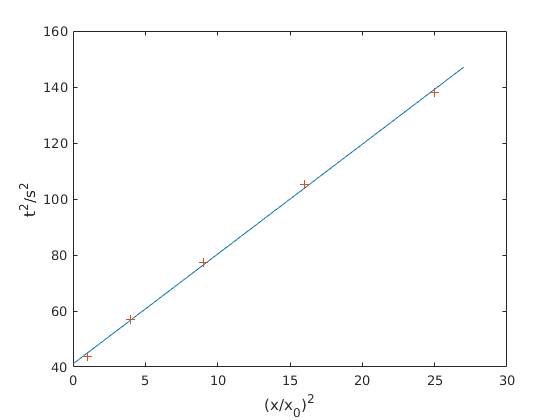
\includegraphics[scale=0.7]{figure_3.png}
	\caption{$t^2$-$x^2$关系图}
\end{figure}

\subsection{实验内容四}

	保持实验条件如下
	
\begin{align*}
	m &= 10.0g \\
	r &= 2.50 cm
\end{align*}

	实验数据如表四所示. \\

\begin{center}
	\begin{longtable}{|c|c|c|c|c|c|c|c|c|c|c|c|c|}

	\caption{第四组实验数据}	\\
	\hline
	$(x_1, x_2)$ & $t_1$/s & $t_2$/s & $t_3$/s & $\bar{t}$/s & $\bar{t}^2/s^2$ \\
	\hline
	$(3, 3')$ & 8.72 & 8.88 & 8.78 & 8.79 & 77.3 \\
	\hline
	$(2, 4')$ & 9.53 & 9.48 & 9.53 & 9.51 & 90.5 \\
	\hline
	$(1, 5')$ & 11.16 & 11.28 & 11.21 & 11.22 & 125.8 \\
	\hline

	\end{longtable}
\end{center}

	可以计算得到
	
\begin{align*}
	\frac{t_2^2 - t_1^2}{t_3^2 - t_1^2} = 0.272 \approx \frac{1}{4}
\end{align*}

\section{分析和讨论}

\subsection{误差来源分析和改进方案}

	实验的主要误差来自于计时的误差和摩擦力矩. 为了尽可能减小摩擦力矩, 实验装置应该注意:
	
\begin{enumerate}
	\item 滑轮与台架距离尽量远, 使绳子与滑轮夹角不致过大.
	\item 刚体的转轴不能夹太紧, 可以适当放松.
	\item 转轴也不能太松, 否则可能不稳定.
	\item 如果摩擦力矩还是太大(比如无法在20s内落地), 可以在转轴的上下固定端用铅笔涂一些石墨减小摩擦力.
	\item 实验前要先用铅垂将转轴$\,OO'\,$调至竖直, 且实验过程中要保证台架位置不变.
\end{enumerate}

	为了减小计时上的误差, 操作上要注意:

\begin{enumerate}
	\item 使砝码每次都从标记处下落, 保证每次下落高度一致.
	\item 如果实验数据起落很大, 应该立即重新测量.
	\item 可以用号牌挡住刚体转动, 保证其在开始转动的时候是静止的.
\end{enumerate}

	为了使实验数据稳定, 可以进行如下操作:

\begin{enumerate}
	\item 台架上的固定螺母要拧紧,保证摩擦力矩$\,M_{\mu}\,$基本不变;
	\item 绕线要密排, 只绕一层, 保持绳子张力的力臂不变(半径最小的槽除外).
	\item 调节滑轮高度使绳子与塔轮转轴垂直.
\end{enumerate}

\subsection{思考题}

	我的实验中确实出现了这个现象. \\
	
	实验二中, 由于有半径很小的线轴, 所以在绕线的时候不得不将线重叠缠绕, 最后导致刚体的力矩可能会大于预期值. 力矩的增大会导致时间变小, 从而导致k过小, 最后导致I过大. 而在实验一中则不会出现这种情况. 

\section{思考和感悟}

	实验原理到操作都不算难, 但是实验的误差很大. 实验仪器非常简单, 如何消除误差就是一个很大的问题. 我们用了很精巧的方案, 比如使用号牌挡住刚体. 也有很多很细致的调节步骤, 比如要把螺丝拧到不紧不松的状态然后实验等等. 我认识到: 实验遇到误差大的时候, 不能总抱怨仪器, 而要从现有的条件出发, 尽可能减小误差!
	
\end{CJK*}
\end{document}
